\chapter{Patterns et descriptions techniques}

\section{Extraction des dates}
L’extraction des dates se fait a l’aide d’expressions régulières que l’on applique au contenu des événements. Nous détectons les dates “standalone” pour marquer le début des événements, mais aussi les intervalles de dates afin de pouvoir préciser une durée d’événement lorsque l’utilisateur se décide à ajouter l’événement au calendrier de son téléphone.

\section{Recyclage de vues dans ListView}
Android fournit des outils pour la gestion des listes graphiques, notamment ListView couplée avec l’interface ListAdapter.\\
ListView est conçue pour être extensible et performante, ce qui signifie:

\begin{enumerate}
\item ListView va essayer d’effectuer des inflations de vues aussi peu que possible.
\item ListView ne va dessiner et disposer ses fils que quand ils sont visibles sur l’écran (ou sur le point de l'être).
\end{enumerate}

Le point 1 se justifie par le fait que les opérations d’inflation de layout sont coûteuses (de l’ordre de 1kB de RAM par vue). Ce problème est résolu par le recyclage des vues non visibles, qu’on appelle \emph{ScrapView}. Cela signifie qu’on peut utiliser des vues recyclées et les mettre à jour, au lieu de faire des inflations de vues pour chaque rangée.

Afin d’implémenter le point 2, ListView utilise un recycleur de vues qui déplacera les vues actives dans une pool recyclable quand elles sortent de l’écran. Ainsi, //TODO

\begin{figure}[h]
  \center
  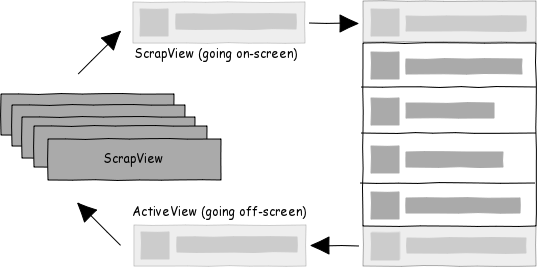
\includegraphics[width=0.92\textwidth]{resources/listview_recycling.png}
\end{figure}

A chaque fois que ListView a besoin d’afficher une nouvelle ligne sur l’écran, elle appelle la méthode \emph{getView()} depuis son adapter.

\begin{adjustbox}{minipage=1.12\textwidth,margin=0pt \smallskipamount,center}
\begin{lstlisting}[style=Java, label=listview1]
public View getView(int position, View convertView, ViewGroup parent)
\end{lstlisting}
\end{adjustbox}

L’argument \emph{convertView} est essentiellement une vue recyclée (\emph{ScrapView}), comme indiqué précédemment. Quand il aura une valeur non nulle, il faudra donc en profiter pour simplement mettre à jour les données au lieu de faire une nouvelle inflation de layout.

\begin{adjustbox}{minipage=1.14\textwidth,margin=0pt \smallskipamount,center}
\begin{lstlisting}[style=Java, label=listview2]
public View getView(int position, View convertView, ViewGroup parent){ 
	View item = mInflater.inflate(R.layout.list_item_icon_text, null);
	((TextView) item.findViewById(R.id.text)).setText(DATA[position]); 
	((ImageView) item.findViewById(R.id.icon)).setImageBitmap(mIcon);
	return item; 
}
\end{lstlisting}
\end{adjustbox}
